%!TEX TS-program=xelatex
\documentclass[xetex]{beamer}

\usefonttheme{professionalfonts}
\usepackage[UTF8]{ctex}
\usepackage{hyperref}
\usepackage{unicode-math}
\usepackage{amsmath, amssymb}
\usepackage{graphicx, wrapfig}
\usepackage{nopageno}

\DeclareMathOperator{\argmax}{argmax}

\usetheme[block=fill, subsectionpage=progressbar]{metropolis}

\setmathfont{XITS Math}

%这是标题页
\title{重积分}
\subtitle{重积分的概念}
\author{数学分析MOOC小组 }
%这是标题页

\begin{document}

\frame{\maketitle}

%这是第一页
\begin{frame}
    \frametitle{曲线网格}

    \begin{figure}[ht]
        \centering %图片居中放置
        % 在这里使用 \includegraphics 插入图片,改变width就可以改变图片的大小。
       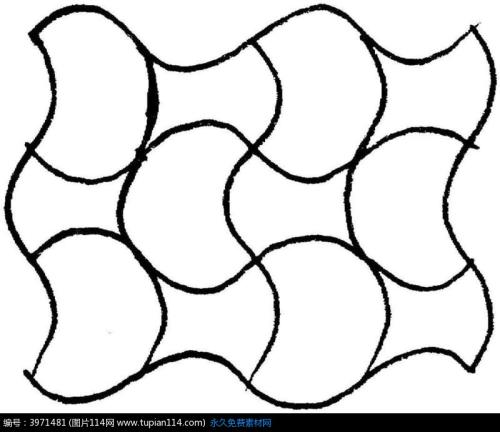
\includegraphics[width=0.7\textwidth]{img/a.jpg}
         \caption{曲线网格示意图}
         \label{fig:identifier}
    \end{figure}

\end{frame}
%这是第一页

%这是第二页
\begin{frame}
    \frametitle{平面图的直径}
    称$S$中所有两点间距离的上确界为$S$的直径,记为$d(s)$,即
    $$d(s)=sup\{r(p_{1},p_{2}) | P_{1} \in S,P_{2} \in S\},$$
    其中$r(P_{1},P_{2})$表示$P_{1}$与$P_{2}$两点间的距离

\end{frame}
%这是第二页

%这是第三页
\begin{frame}
    \frametitle{重积分的定义}
    设$D$是平面上可求面积的有界闭区域,$f(x,y)$定义在$D$上,用任意曲线网格将$D$分成有限个可求面积的区域$\Delta\sigma_{1},\Delta\sigma_{2},....\Delta\sigma_{n}$(称为D的一个分法),任取$(\xi_{i},\eta_{i})\in\Delta\sigma_{i},\Delta\sigma_{i}$既表示小块平面区域,也表示小块区域的面积,作和
     $$\sigma = \sum_{i=1}^{n}{f(\xi_{i},\eta_{i})\Delta\sigma_{i}}$$
     记$d(i)$为$\Delta\sigma_{i}$的直径,$\lambda = \max\limits_{1\leq i \leq n}|d_{i}|.$如果当$\lambda\rightarrow0$时,$\sigma$的极限存在,则称$f(x,y)$在$D$可积,并称极限值为$f(x,y)$在$D$的二重积分,记为
     \begin{center}
     $\iint\limits_Df(P)d\sigma$或$\iint\limits_Df(x,y)dxdy.$
     \end{center}
\end{frame}
%这是第三页

%这是第三‘页
\begin{frame}
    \frametitle{重积分的定义}
    也就是说,
    $$\iint\limits_Df(x,y)dxdy = \iint\limits_Df(P)d\sigma = \lim\limits_{\lambda\rightarrow0}\sum_{i=1}^{n}{f(\xi_i,\eta_i)\Delta\sigma_i}$$
\end{frame}
%这是第三’页
    

%这是第四页
\begin{frame}
    \frametitle{重积分的几何意义}
    \begin{figure}[ht]
        \centering %图片居中放置
        % 在这里使用 \includegraphics 插入图片,改变width就可以改变图片的大小。
       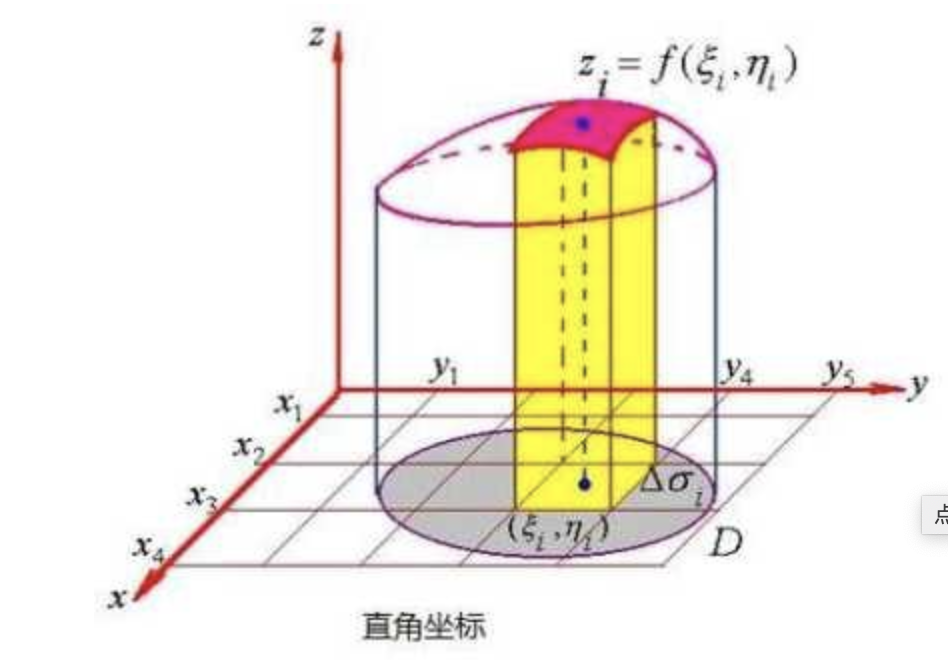
\includegraphics[width=0.7\textwidth]{img/b.jpg}
         \caption{重积分的几何意义是立体图形的体积}
         \label{fig:identifier}
    \end{figure}
\end{frame}
%这是第四页

%这是第五页
\begin{frame}
    \frametitle{重积分的基本性质}
    (1)若$f(P)$在$D$可积,$k$为常数,则$kf(P)$也在$D$可积,且
    $$\iint\limits_Dkf(P)d\sigma = k\iint\limits_Df(P)d\sigma.$$
    
    (2)若$f(P),g(P)$都在$D$可积,则$f(P) \pm g(P),f(P)g(P)$也在$D$可积,并且
    $$\iint\limits_D[f(P) \pm g(P)]d\sigma=\iint\limits_Df(P)d\sigma \pm \iint\limits_Dg(P)d\sigma.$$
\end{frame}
%这是第五页

%这是第六页
\begin{frame}
    \frametitle{重积分的基本性质}
    (3)(可加性)若$D$由$D_1,D_2$组成$:D = D_1 \cup D_2,$且$D_1,D_2$除边界外不相交,则$f(P)$在$D$可积的充要条件是$f(P)$在$D_1,D_2$均可积,且
    $$\iint\limits_Df(P)d\sigma = \iint\limits_{D_1}f(P)d\sigma + \iint\limits_{D_2}f(P)d\sigma$$
    
    (4)(单调性)若$f$与$g$都在$D$可积,且在$D$的每点$P$都有$f(P) \leq g(P),$则
    $$\iint\limits_Df(P)d\sigma\leq\iint\limits_Dg(P)d\sigma.$$
\end{frame}
%这是第六页

%这是第七页
\begin{frame}
    \frametitle{重积分的基本性质}
    (5)若$f(P)$在$D$可积,则$|f(P)|$也在$D$可积,并且
    $$| \iint \limits_Df(P)d \sigma | \leq \iint \limits_D|f(P)|d \sigma.$$
    (6)(积分中值定理)设$D$是有界闭区域(因而是连通的),$f(P)$在$D$上连续,则存在$P_0 \in D,$使得
    $$\iint\limits_Df(P)d\sigma=f(P_0)|D|$$
    其中$|D|$表示$D$的面积
\end{frame}
%这是第七页

%这是第八页
\begin{frame}
    \frametitle{例题}
    \begin{figure}[ht]
        \centering %图片居中放置
        % 在这里使用 \includegraphics 插入图片,改变width就可以改变图片的大小。
       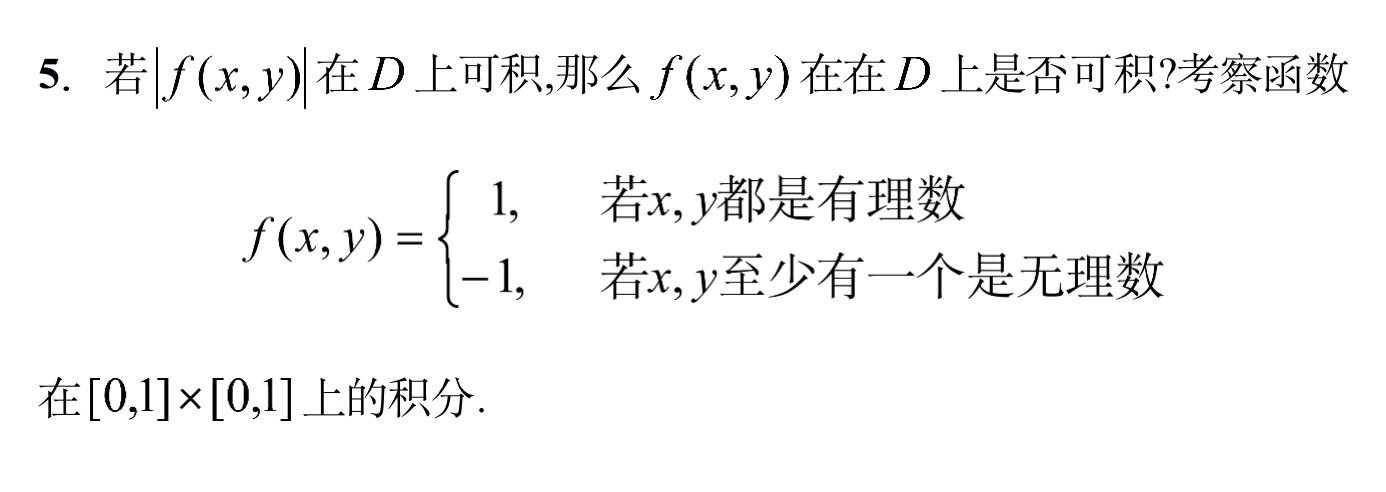
\includegraphics[width=1.0\textwidth]{img/c.jpg}
    \end{figure}
\end{frame}
%这是第八页

%这是第九页
\begin{frame}
    \frametitle{解答过程}
    \begin{figure}[ht]
        \centering %图片居中放置
        % 在这里使用 \includegraphics 插入图片,改变width就可以改变图片的大小。
       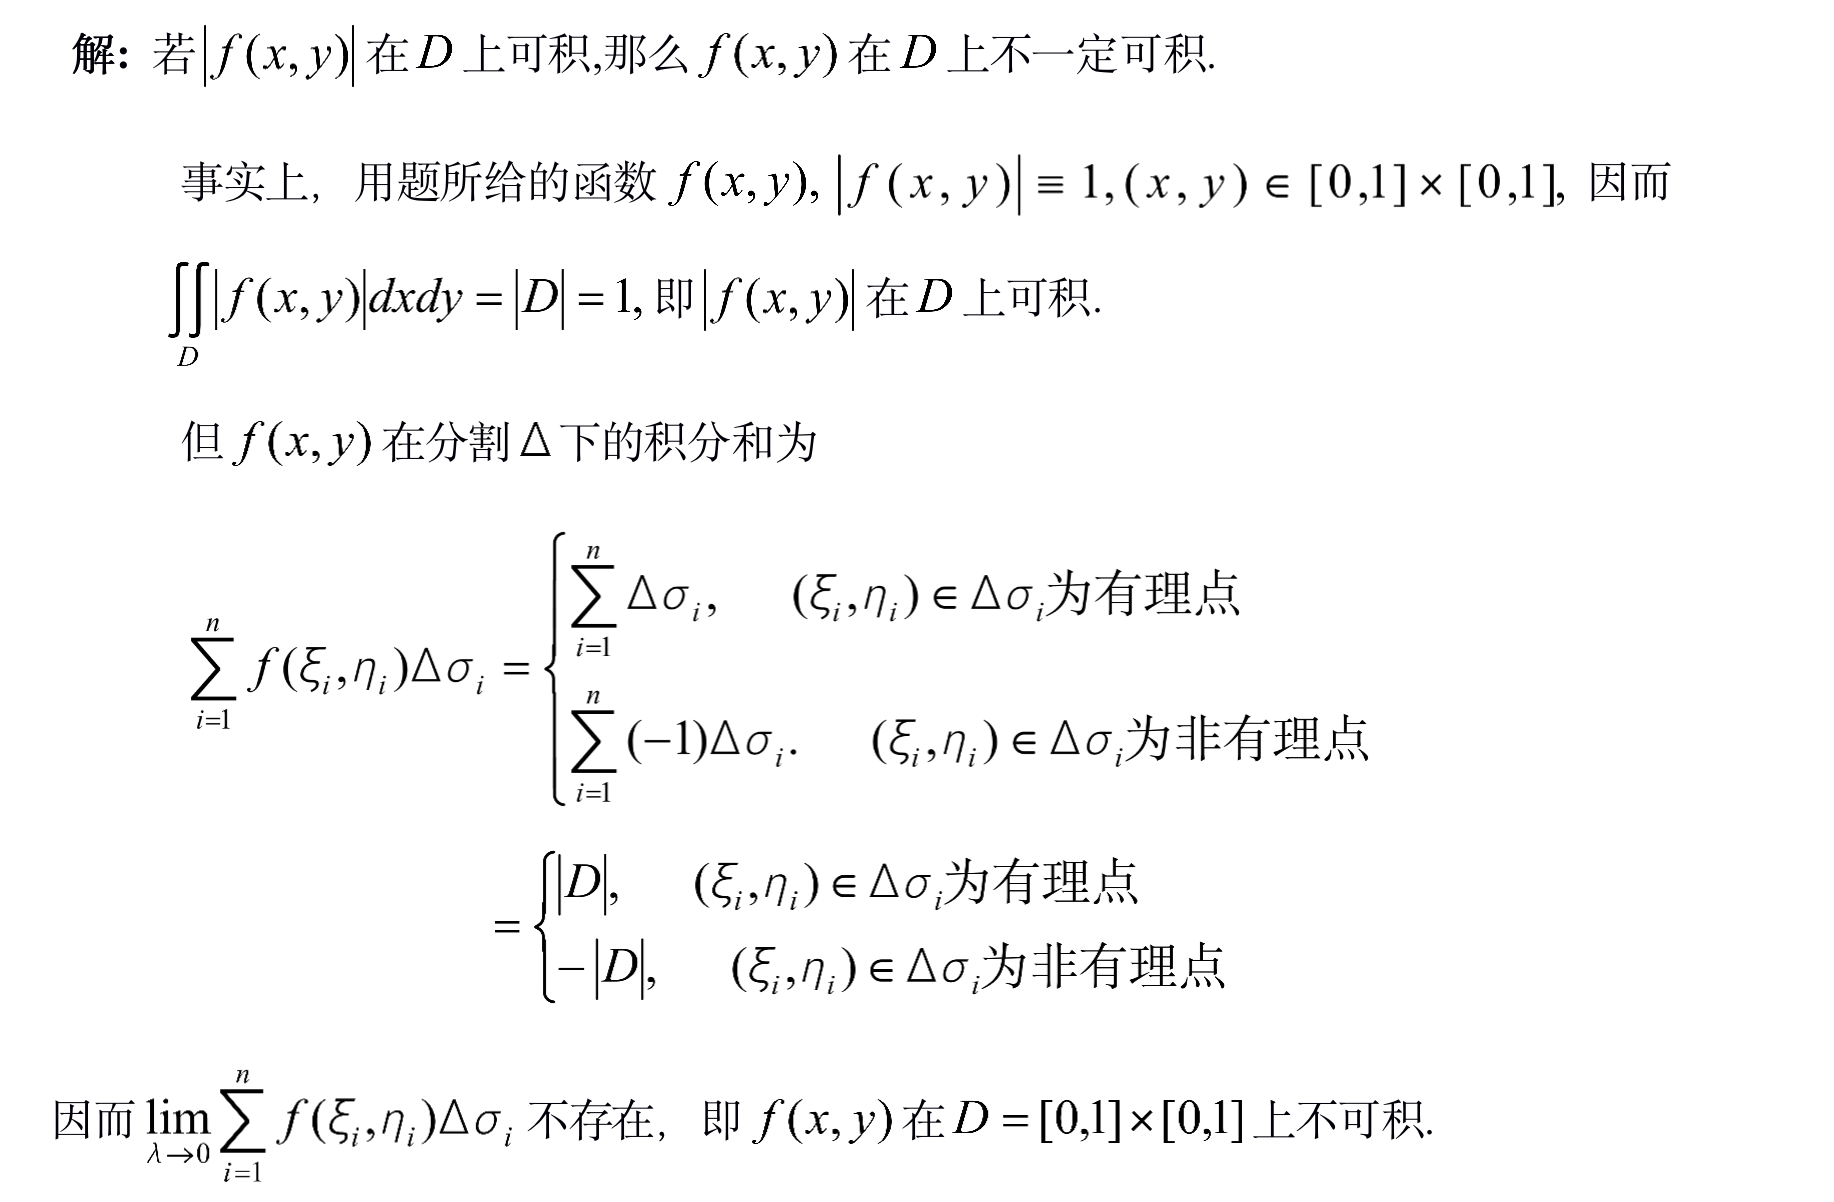
\includegraphics[width=1.0\textwidth]{img/d.jpg}
    \end{figure}
\end{frame}
%这是第九页

\section{感谢观看!}

\end{document}